\documentclass{sigplanconf}
\usepackage{graphicx}
\graphicspath{{image/}}
\DeclareGraphicsExtensions{.png}

% The following \documentclass options may be useful:

% preprint      Remove this option only once the paper is in final form.
% 10pt          To set in 10-point type instead of 9-point.
% 11pt          To set in 11-point type instead of 9-point.
% authoryear    To obtain author/year citation style instead of numeric.

\usepackage{amsmath}


\begin{document}

\special{papersize=8.5in,11in}
\setlength{\pdfpageheight}{\paperheight}
\setlength{\pdfpagewidth}{\paperwidth}

\conferenceinfo{CONF 'yy}{Month d--d, 20yy, City, ST, Country} 
\copyrightyear{2016} 
\copyrightdata{978-1-nnnn-nnnn-n/yy/mm} 
\doi{nnnnnnn.nnnnnnn}

% Uncomment one of the following two, if you are not going for the 
% traditional copyright transfer agreement.

%\exclusivelicense                % ACM gets exclusive license to publish, 
                                  % you retain copyright

%\permissiontopublish             % ACM gets nonexclusive license to publish
                                  % (paid open-access papers, 
                                  % short abstracts)

\titlebanner{Rapid Information Factory}        % These are ignored unless
\preprintfooter{short description of paper}   % 'preprint' option specified.

\title{Rapid Information Factory}
\subtitle{Applying Lean Six Sigma to Parallel Processsing Framework}

\authorinfo{Andreas Francois Vermeulen}
           {University of St Andrew and University of Dundee}
           {afvermeulen@dundee.ac.uk}
\authorinfo{Dr Vladimir Janjic \and Prof Janet Hughes}
           {University of St Andrew \and University of Dundee}
           {jhughes@computing.dundee.ac.uk \and vj32@st-andrews.ac.uk}

\maketitle

\begin{abstract}
This is the text of the abstract.
\end{abstract}

\category{CR-number}{subcategory}{third-level}

% general terms are not compulsory anymore, 
% you may leave them out
\terms
Parallel applications and frameworks, lean six sigma

\keywords
rapid information factory, rif, framework, lean six sigma, heterogeneous computing, parallel, beowulf, cluster, master-slave, pipe-line.

\section{Introduction}
The Rapid Information Factory is a data processing architecture that enables the enhanced processing of data by using a structured and highly optimised parallel processing framework. The core of the framework is a processing pipeline with feedback to enhance the processing of the the data into information. Our research covers the structure of this processing framework and the use of a three node Beowulf cluster \cite{sterling2002beowulf} that combines into the formation of the Rapid Information Factory. The improve the performance of the factory we apply same Lean Six Sigma \cite{george2005lean} rules that applies to normal manufacturing factories with proven success.
\section{Research Question}
"Does a Rapid Information Factory improve prosessing of data into information when Lean Six Sigma improvements normally applied to manufactoring factories is used to guide improvements?"
\section{Background}
The following is the backgound research for this presentation.
\subsection{Lean work cells}
The Lean work cells \cite{black2003lean} is an optimised processing unit that performs work with singlular work outcome. The factory is built up using various manufacturing processes joint to form work cells that delivers the works on a just-in-time processing principal \cite{cheng1996just}.
The lean work cells directly translate into a FastFlow Farm \cite{aldinucci2009fastflow} that enables the formation of a optimised processing unit.
\section{Lean Waste}
A waste is any step or action in a process that is not required to complete a process (i.e. “Non Value-Adding”) successfully. When Waste is eliminate, only the steps that are required (i.e. “Value-Adding”) to deliver a satisfactory product or service to the customer remain in the process.
\subsection{Eight Lean Wastes}
The lean wastes are categorise into eight wastes type.
These are the 8 Wastes:
\begin{enumerate}
  \item Defects : Products or services that are out of specification that require resources to correct.
  \item Overproduction : Producing too much of a product before it is ready to be sold;
  \item Waiting for the previous step in the process to complete.
  \item Non-Utilized Talent – Employees that are not effectively engaged in the process.
  \item Transportation – Transporting items or information that is not required to perform the process from one location to another.
  \item Inventory or information that is sitting idle (not being processed).
  \item Motion – People, information or equipment making unnecessary motion due to workspace layout, ergonomic issues or  searching for misplaced items.
  \item Extra Processing – Performing any activity that is not necessary to produce a functioning product or service.
\end{enumerate}
\begin{figure}
  \centering
  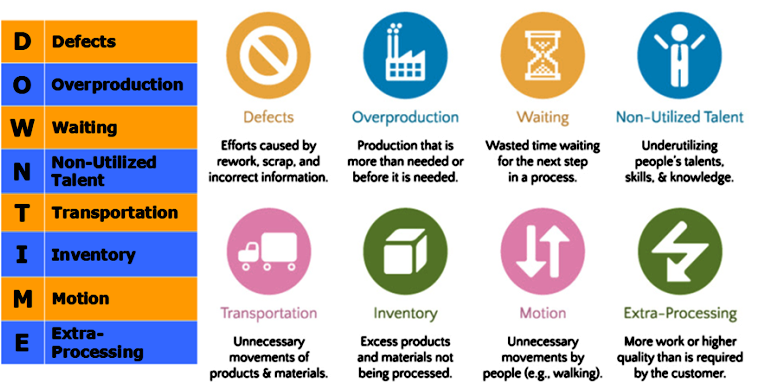
\includegraphics[width=8cm]{lean8wastes}
  \caption{Eight Lean Wastes}
\end{figure}
\section{5S}

The 5S is a workplace organization technique composed for five primary phases: Sort, Set In Order, Shine, Standardize, and Sustain.

\begin{figure}
  \centering
  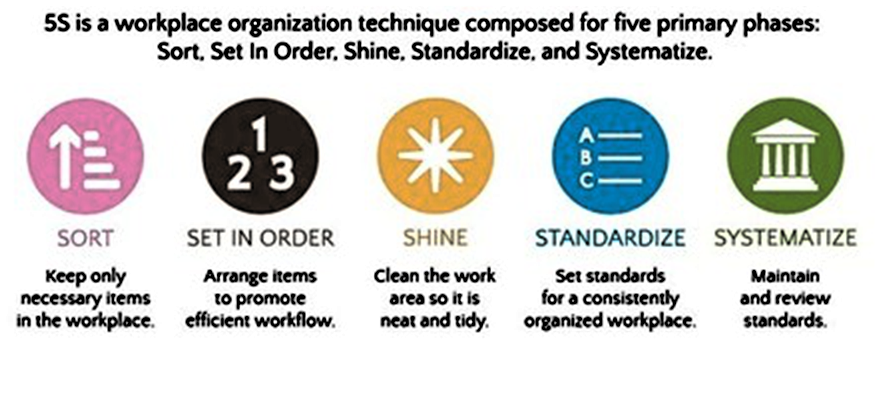
\includegraphics[width=8cm]{5s}
  \caption{5S - Sort, Set In Order, Shine, Standardize, and Sustain.}
\end{figure}

Sort – Keep only necessary items in the workplace.

    Review tools, parts, and instructions;
    Keep only what is essential;
    Eliminate anything that is non-essential.

Examples: Obsolete or expired procedures, damaged or expired inventory, defunct or old equipment

Set In Order – Arrange items to promote efficient work flow.

    Arrange items in a logical order;
    Indicate places for each item clearly;
    Keep each item close to where it will be used.

Reduces: excess movement, excess transportation, over processing, over production, excess inventory, excess delays, defects

Shine – Clean the work area so it is neat and tidy.

    Make cleaning a part of daily work;
    Assign areas of responsibility;
    Return all items or files to their assigned place.

Examples: Dirty tools and equipment, spills and leaks, clutter and mess

Standardize – Set standards for a consistently organized workplace.

    Create standards for Sort, Set In Order, and Shine;
    Make standards easy to understand with Visual Controls;
    Assign and educate on individual responsibilities.

Examples: Work instructions, hazard warnings, equipment/tool labels, process diagrams

Sustain – Maintain and review standards.

    Measure and monitor process;
    Address root causes and avoid reversion to the “old ways”;
    Promote individual feedback and response for improvement.

\subsection{Poka-Yoke}
Poka-yoke is a Japanese term that means “mistake-proofing”. A poka-yoke is any mechanism in a Lean Manufacturing process that helps an equipment operator avoid (yokeru) mistakes (poka). Its purpose is to eliminate product defects by preventing, correcting, or alert to errors as they occur.

\subsection{Takt Time}
The Takt Time is the rate at which a finished product needs to be completed in order to meet customer demand.

\subsection{Cycle Time}
The time it takes to do one repetition of any particular task typically measured from “Start to Start” the starting point of one product’s processing in a specified machine or operation until the start of another similar product’s processing in the same machine or process. 

\section{Software - Building Block}

\subsection{0QM}
The system uses the ZeroQM \cite{hintjens2011omq} libraries to communicate beteen the processes in the work cells.

ZeroMQ supplies:
\begin{itemize}
  \item Connect your code in any language, on any platform.
  \item Carries messages across inproc, IPC, TCP, TIPC, multicast.
  \item Smart patterns like pub-sub, push-pull, and router-dealer.
  \item High-speed asynchronous I/O engines, in a tiny library.
  \item Supports multi language and multi platform.
  \item Build various architectures: centralised or distributed.
\end{itemize}

\subsection{C++}

The system is developed using C++.

\section{Rapid Information Factory}
The factory is a singular processing solution that processes all data into information using a XML based rules. The solution consists of an interaction between three dimensional frameworks:
\subsection{Customer Framework}
This is the view the single view of the information to the customer. It is structured to show the information in the view the customer spesifies in the functional requirements. As for this spesific research this is not expanded or discussed further.
\subsection{Project Framework} 
The factory evolves over time as it is developed and then redeveloped to handle extra enhancements or new data sources. The project is driven by a agile project methodology consisting a backlog and a cycle of five day sprints covering a period of six months. As for this spesific research this is not expanded or discussed further.
\subsection{Rapid Information Factory Framework}
The processing farmework is an ontology scripting the processes in Extensible Markup Language (XML) to define the set of rules for encoding the process and the interactions between process. The framework consists of a five high-level layers:
\begin{figure}
  \centering
  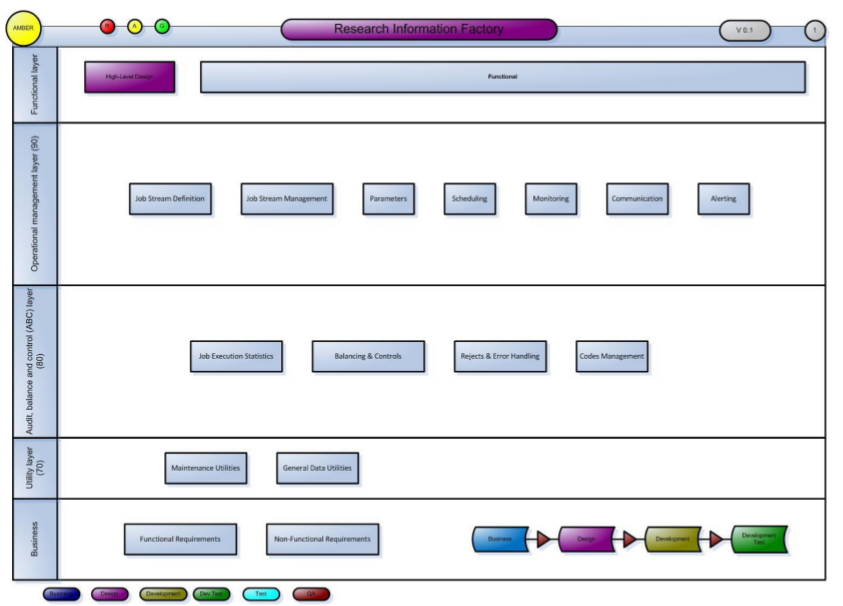
\includegraphics[width=8cm]{RIFF1}
  \caption{Rapid Information Factory Framework}
\end{figure}
\subsubsection{Business Layer}
The Business Layer contains the Business spesific framework configurations that covers either functional requirements or non-functional requirements. The layer consists of two groupings:
\begin{enumerate}
  \item Functional work cell
  \item Non-functional work cell
\end{enumerate}
As for this spesific research this is not expanded or discussed further.
\subsubsection{Utility Layer}
The Untility Layer consists of sets of utilities for the overall factory. The layer consists of two groupings of utilities:
\begin{enumerate}
  \item Maintance utility work cell
  \item General utility work cell
\end{enumerate}
As for this spesific research this is not expanded or discussed further.
\subsubsection{Audit, Balance and Control Layer}
The Audit, Balance and Control Layer (ABC) is the layer that supports the factory while it is running.
This layer handles any active processing allowcated to the Beowulf engine.
The layer consists of three groupings.
\begin{enumerate}
  \item Audit work cell
  \item Balance work cell
  \item Control work cell
\end{enumerate}
\subsubsection{Operational Management Layer}
The Operational Management Layer supports setup of the individual job definition and 
interaction between jobs, job parameters, scheduling, monitoring, communication and alerting within the factory. The layer is the central management engine of the factory. The layer consists of five groupings:
\begin{enumerate}
  \item Jobs work cell
  \item Schedule work cell
  \item Monitor work cell
  \item Communication work cell
  \item Alerts work cell
\end{enumerate}
\subsubsection{Functional Layer}
The functional layer store the scripts that describes every functional process of the complete factory.
\begin{figure}
  \centering
  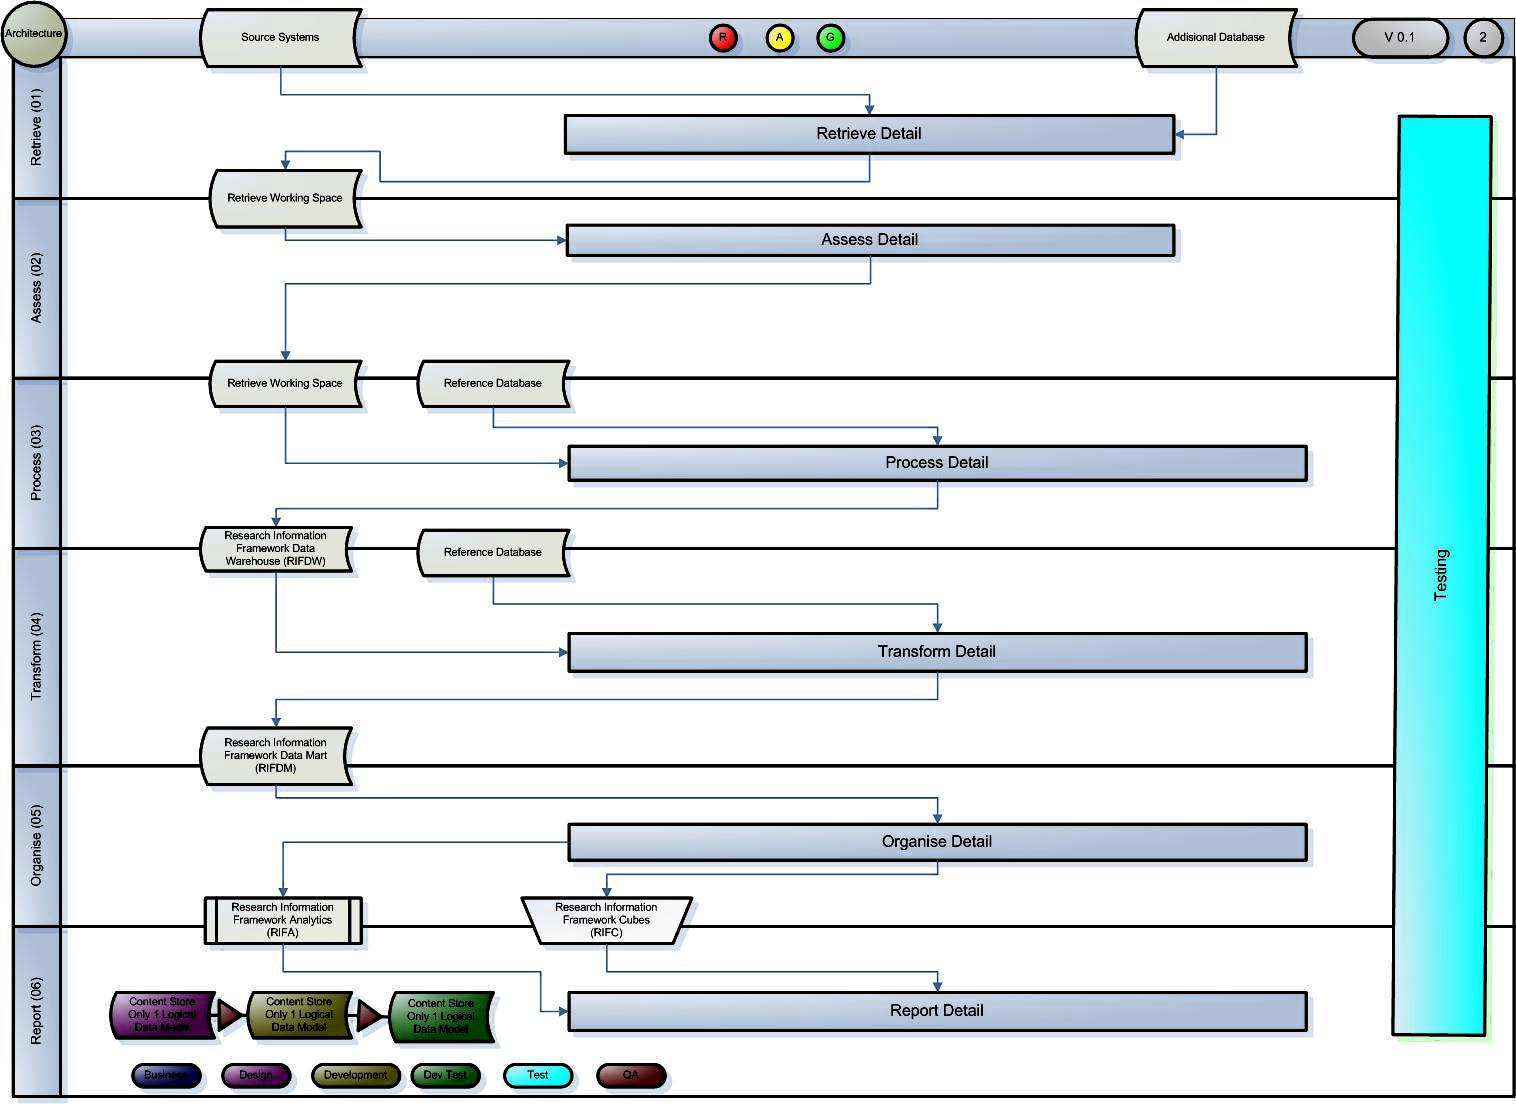
\includegraphics[width=8cm]{RIFF2}
  \caption{R-A-P-T-O-R process pipe}
\end{figure}
The layer consists of six groupings of jobs:
\begin{enumerate}
  \item Retrieve work cell
  \item Assess work cell
  \item Process work cell
  \item Transform work cell
  \item Organise work cell
  \item Report work cell
\end{enumerate}
\subsection{Audit, Balance and Control Layer}
The Audit, Balance and Control Layer (ABC) is the layer that supports the factory while it is running.
This layer handles any active processing allowcated to the Beowulf engine. The layer consists of three groupings.
\subsubsection{Audit work cell}

\subsubsection{Balance work cell}

\subsubsection{Control work cell}

\subsection{Operational Management Layer}
The Operational Management Layer supports setup of the individual job definition and 
interaction between jobs, job parameters, scheduling, monitoring, communication and alerting within the factory. The layer is the central management engine of the factory. The layer consists of five groupings:
\subsubsection{Jobs work cell}

\subsubsection{Schedule work cell}

\subsubsection{Monitor work cell}

\subsubsection{Communication work cell}

\subsubsection{Alerts work cell}

\subsection{Functional Layer}
The functional layer store the scripts that describes every functional process of the complete factory. The layer consists of six groupings of jobs:
\subsubsection{Retrieve work cell}

\subsubsection{Assess work cell}


\subsubsection{Process work cell}

\subsubsection{Transform work cell}

\subsubsection{Organise work cell}

\subsubsection{Report work cell}

\appendix
\section{Performance Improvement Results}
The Performance Improvement Results is as follows:
Applying 5S - Sort improvement process to Retrieve Jobs.
Applying 5S - Set-in-Order improvement process to Retrieve Jobs.
Applying 5S - Shine improvement process to Retrieve Jobs.
Applying 5S - Standardise Sort improvement process to Retrieve Jobs.
Applying 5S - Sustain improvement process to Retrieve Jobs.
Applying Lean Waste - Transport to Retrieve Jobs.
Applying Lean Waste - Inventory to Retrieve Jobs.
Applying Lean Waste - Motion to Retrieve Jobs.
Applying Lean Waste - Waiting to Retrieve Jobs.
Applying Lean Waste - Overproduction to Retrieve Jobs.
Applying Lean Waste - Over-processing to Retrieve Jobs.
Applying Lean Waste - Defects to Retrieve Jobs.

\acks

Thank you to Prof Mark Whitehorn and Prof Janet Hughes for her guidance into the Operational Research, Business Intelligence, Data Science and Data Engineering concepts utilised in this research.

% We recommend abbrvnat bibliography style.

\bibliographystyle{abbrvnat}

% The bibliography should be embedded for final submission.

\bibliography{andre}
\softraggedright

\end{document}

%                       Revision History
%                       -------- -------
%  Date         Person  Ver.    Change
%  ----         ------  ----    ------

%  2015.06.01   AV      0.1--1  First draft
